\section{Tiền xử lý dữ liệu}
\subsection{Truy xuất dữ liệu đầu vào}
    Dữ liệu đầu ra ở bước này là kích thước mẫu số liệu, kiểu dữ liệu. \\
    Ta sử dụng các tập lệnh (command): 
    \begin{enumerate}
        \item nrow(): xác định số lượng dòng (row).
        \item ncol(): xác định số lượng cột (column).
        \item head(): xác định các dòng đầu tiên của bảng số liệu.
        \item str(): xác định tổng quát cấu trúc của đối tượng.
    \end{enumerate}

    Phần code lập trình xử lý các thông số về kích thước:

    \begin{lstlisting}
    library(readr)
    dirty_data <- read_csv("dirty_data.csv", show_col_types = FALSE)
    cat("Rows:", nrow(dirty_data), "Columns:", ncol(dirty_data), "\n")
    print(head(dirty_data))
    str(dirty_data)
    \end{lstlisting}

    Kết quả thu được: \\
    Dữ liệu số dòng và số cột: 500 dòng, 16 cột.
    \begin{figure}[htbp]
        \centering
        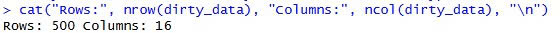
\includegraphics[width=0.8\linewidth]{Image/Chapter_3/hinh_1}
        \caption{Kết quá thể hiện số dòng và cột.}
        \label{Ket_qua_the_hien_so_dong_va_cot}
    \end{figure}

    Dữ liệu của một số dòng đầu tiên của dữ liệu:
    \begin{figure}[htbp]
        \centering
        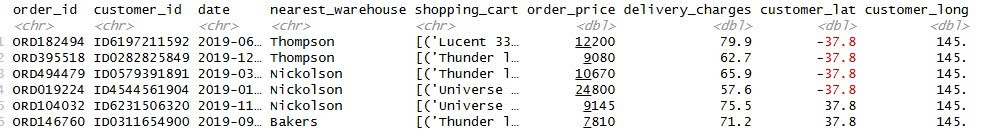
\includegraphics[width=1\linewidth]{Image/Chapter_3/hinh_2}
        \caption{Kết quá thể hiện các dòng đầu tiên.}
        \label{Ket_qua_the_hien_dong_dau_tien}
    \end{figure}

\subsection{Xác định các biến cần thiết}
    Sau khi xác định được các thông số đầu vào, ta cần giữ lại các biến cố định phụ vụ cho việc phân tích số liệu và thống kê.
    Ta sử dụng các tập lệnh (command):
    \begin{enumerate}
        \item c(): tạo vector chuỗi ký tự chứa danh sách các biến cần thiết.
        \item new\_df <- df[rows, columns]: trích xuất 1 phần dữ liệu từ df sang new\_df trong khoảng [rows] và [columns].
        \item names(): trích xuất các biến hiện có trong dữ liệu.
    \end{enumerate}

    \begin{lstlisting}
    selected_vars <- c("nearest_warehouse", "delivery_charges", "coupon_discount", "order_total", "season", "is_expedited_delivery", "distance_to_nearest_warehouse", "is_happy_customer", "customer_lat", "customer_long", "order_price")
    new_data <- dirty_data[, selected_vars]
    cat("Rows:", nrow(new_data), "Columns:", ncol(new_data), "\n")
    print(names(new_data))
    \end{lstlisting}

    Kết quả thu được: \\
    Dữ liệu mới sau khi xác định các biến cần thiết là: 500 dòng, 11 cột.
    \begin{figure}[htbp]
        \centering
        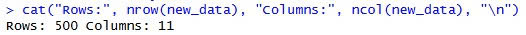
\includegraphics[width=0.8\linewidth]{Image/Chapter_3/hinh_3}
        \caption{Kết quá thể hiện các dòng và cột sau khi loại bỏ các biến.}
        \label{Ket_qua_the_hien_dong_va_cot_sau_khi_loai_bo_cac_bien}
    \end{figure}

    Từ đó, ta xác định được các biến cần thiết:
    \begin{figure}[htbp]
        \centering
        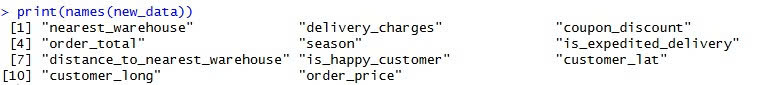
\includegraphics[width=1\linewidth]{Image/Chapter_3/hinh_4}
        \caption{Kết quá thể hiện tên các biến cần thiết.}
        \label{Ket_qua_the_hien_ten_cac_bien_can_thiet}
    \end{figure}

    Vì mục tiêu sau khi xử lý dữ liệu đầu vào được dùng để phân tích và thống kê liên quan đến phí giao hàng:
    \begin{itemize}
        \item[] \textbf{Các biến được loại bỏ:} các biến mang tính danh định và mang tính phân loại trong việc giao hàng: "order\_id", "customer\_id", "date", "shopping\_cart" và "date". 
        \item[] \textbf{Các biến cần được giữ lại:} 
            \begin{enumerate}
                \item nearest\_warehouse: xác định kho gần nhất.
                \item delivery\_charges: xác định cước phí giao hàng.
                \item coupon\_discount: số tiền được giảm.
                \item order\_total: tổng số tiền của đơn gian.
                \item season: mùa mà đơn hàng được giao.
                \item is\_expedited\_delivery: sự khác biệt giữa đơn giao nhanh và giao bình thường.
                \item distance\_to\_nearest\_warehouse: khoảng cách giữa kho hàng so với nơi nhận.
                \item is\_happy\_customer: thái độ của khách hàng khi nhận đơn
                \item customer\_lat: vĩ độ của nơi nhận.
                \item customer\_long: kinh độ của nơi nhận.
                \item order\_price: giá tiền của đơn hàng có ảnh hưởng đến xu hướng của đơn giá.
            \end{enumerate}
    \end{itemize}

\subsection{Kiểm tra thiếu dữ liệu, chuẩn hoá dữ liệu, kiểm tra công thức}
    Sau khi có được các dữ liệu cần thiết cho việc phân tích phí giao hàng (delivery charges), dữ liệu phải được kiểm tra và chỉnh sửa những lỗi như: biến thiếu dữ liệu, biến phụ thuộc công thức, dữ liệu dạng chuỗi (string) phải được chuẩn hoá định dạng.
    \subsubsection{Kiểm tra giá trị thiếu}
        Ta sử dụng các lệnh (command):
        \begin{enumerate}
            \item is.na(): kiểm tra dữ liệu đưa vào, trả về ma trận giá trị TRUE (nếu giá trị là NA (Not Available)) và FALSE (nếu có giá trị).
            \item apply(is.na(new\_data), 2, sum): tổng từng cột, trả về giá trị các ô có giá trị là NA.
            \item sapply(new\_data, function(x) if (is.character(x)) sum(trimws(x) == "", na.rm = TRUE) else 0): kiểm tra xem ô đó phải là chuỗi và "" hay " " không, đếm tất cả các ô chuỗi rỗng đó.
            \item for (col in names(new\_data)): duyệt qua từng cộng của new\_data.
            \item is.character(new\_data[[col]]): chỉ duyệt những cột có kiểu dữ liệu là dạng chuỗi (string).
            \item which(): tìm vị trí dòng của ô được duyệt đến.
            \item new\_data[[col]][empty\_index] <- NA: quy chuẩn các giá trị thiếu vào mục NA (Not Available).
        \end{enumerate}

        \begin{lstlisting}
    missing_before <- apply(is.na(new_data), 2, sum)
    empty_before <- sapply(new_data, function(x) if (is.character(x)) sum(trimws(x) == "", na.rm = TRUE) else 0)
    print(missing_before)
    print(empty_before)
    for (col in names(new_data)) {
    if (is.character(new_data[[col]])) {
        empty_index <- which(trimws(new_data[[col]]) == "")
        new_data[[col]][empty_index] <- NA
    }
    }
    rows_before_missing <- nrow(new_data)
    new_data <- na.omit(new_data)
    cat("Rows removed:", rows_before_missing - nrow(new_data), "\n")
        \end{lstlisting}

        Kết quả thu được: \\
        Sau khi phân tích các lỗi thiếu, chuẩn hoá các dạng thiếu, khoảng trống thành dạng NA, ta loại bỏ được 0 dòng bị thiếu, điều này chứng tỏ rằng dữ liệu đầu vào có đủ dữ liệu cho từng biến.
        \begin{figure}[htbp]
            \centering
            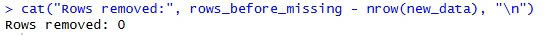
\includegraphics[width=0.8\linewidth]{Image/Chapter_3/hinh_5}
            \caption{Kết quá thể hiện 0 dòng được xoá.}
            \label{Ket_qua_the_hien_ten_0_dong_duoc_xoa}
        \end{figure}

        \subsubsection{Chuẩn hoá định dạng dữ liệu}
        Sau khi xử lý các giá trị bị thiếu, dữ liệu đầu vào vẫn còn các lỗi như thiếu đồng bộ giữa ký tự chuỗi hoa và ký tự chuỗi thường trong cột "nearest\_warehouse" và "season", thế nên, bộ dữ liệu cần được xử lý chuẩn hoá định dạng.
        Ta sử dụng các lệnh (command):
        \begin{enumerate}
            \item unique(): trích xuất ra giá trị phân biệt (không lặp lại) trong dữ liệu.
            \item trimws(): cắt bỏ các khoảng trắng thừa ở hai đầu chuỗi ký tự.
            \item tolower(): chuyển dạng chuỗi ký tự về dạng thường.
            \item unname(): loại bỏ nhãn tên, chỉ giữ lại chuỗi.
        \end{enumerate}

        \begin{lstlisting}
    print(unique(new_data$nearest_warehouse))
    print(unique(new_data$season))
    warehouse_map <- c(thompson = "Thompson", nickolson = "Nickolson", bakers = "Bakers")
    warehouse_key <- tolower(trimws(new_data$nearest_warehouse))
    new_data$nearest_warehouse <- unname(warehouse_map[warehouse_key])
    season_map <- c(spring = "Spring", summer = "Summer", autumn = "Autumn", winter = "Winter")
    season_key <- tolower(trimws(new_data$season))
    new_data$season <- unname(season_map[season_key])
    print(table(new_data$nearest_warehouse))
    print(table(new_data$season))
        \end{lstlisting}

        Kết quả thu được: \\
        Sau khi xử lý và trích xuất ký tự in hoa và in thường, ta được các kết quả như sau:
        \begin{figure}[htbp]
            \centering
            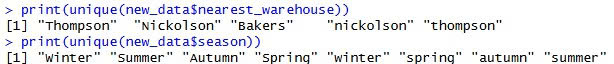
\includegraphics[width=0.8\linewidth]{Image/Chapter_3/hinh_6}
            \caption{Kết quá thể hiện các giá trị unique.}
            \label{Ket_qua_the_hien_ten_cac_gia_tri_unique}
        \end{figure}
        
        Sau khi đã chuẩn hoá các ký tự theo key, ta có thể đưa ra số liệu về tổng đơn hàng ở từng kho và từng mùa. 
        \begin{figure}[htbp]
            \centering
            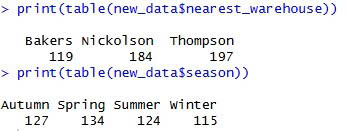
\includegraphics[width=0.6\linewidth]{Image/Chapter_3/hinh_7}
            \caption{Kết quá thể hiện số lần tên các kho hàng và mùa mua hàng.}
            \label{Ket_qua_the_hien_so_lan_ten_cac_kho_hang_va_mua_mua_hang}
        \end{figure}

    \subsubsection{Kiểm tra công thức tính tổng tiền và chỉnh sửa sai số}
        Sau khi đã xử lý các vấn đề về việc thống nhất định dạng dữ liệu, ta cần xử lý sự chính xác mối liên hệ giữa những biến trong dữ liệu. Trong đó, biến "order\_total" có mối liên hệ với các biến còn lại.

        Cụ thể, biến "order\_total" được tính như sau:
        \begin{equation*}
            \text{order\_total} = \text{order\_price} \times \left(1 - \frac{\text{coupon\_discount}}{100}\right) + \text{delivery\_charges}
            \label{eq:order_total}
        \end{equation*}

        \begin{lstlisting}
    new_data$calculated_total <- new_data$order_price * (1 - new_data$coupon_discount / 100) + new_data$delivery_charges
    mismatch_before <- sum(abs(new_data$order_total - new_data$calculated_total) > 0.01)
    cat("Rows outside tolerance before correction:", mismatch_before, "\n")
    new_data$order_total <- new_data$calculated_total
    mismatch_after <- sum(abs(new_data$order_total - new_data$calculated_total) > 0.01)
    cat("Rows outside tolerance after correction:", mismatch_after, "\n")
        \end{lstlisting}

        Kết quả thu được: \\
        Số lỗi (giá trị không khớp với công thức) trước khi sửa chữa:
        \begin{figure}[htbp]
            \centering
            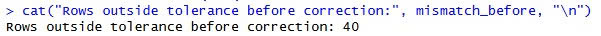
\includegraphics[width=0.8\linewidth]{Image/Chapter_3/hinh_8}
            \caption{Kết quá thể hiện số giá trị lệch.}
            \label{Ket_qua_the_hien_so_gia_tri_lech}
        \end{figure}

        Số lỗi sau khi đã áp dụng và đối sánh với lý thuyết công thức:
        \begin{figure}[htbp]
            \centering
            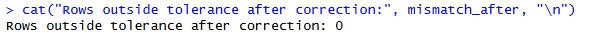
\includegraphics[width=0.8\linewidth]{Image/Chapter_3/hinh_9}
            \caption{Kết quá thể hiện số giá trị lệch sau khi sửa.}
            \label{Ket_qua_the_hien_so_gia_tri_lech_sau_khi_sua}
        \end{figure}

        Sau khi dữ liệu được xử lý và kiểm duyệt, ta có thể xoá cột "calculated\_total" (biến trung gian cho việc kiểm duyệt chính xác) và xuất đầu ra tập tin dữ liệu sạch "clean\_data.csv"
        \begin{lstlisting}
    new_data$calculated_total <- NULL
    write_csv(new_data, "clean_data.csv")
        \end{lstlisting}
        